%% ****** Start of file apstemplate.tex ****** %
\documentclass[aps,prl,reprint,groupedaddress]{revtex4-2}

% You should use BibTeX and apsrev.bst for references
% Choosing a journal automatically selects the correct APS
% BibTeX style file (bst file), so only uncomment the line
% below if necessary.
% \bibliographystyle{apsrev4-2}

\usepackage{graphicx}
\usepackage{epstopdf}
\usepackage{amsmath}
\usepackage{amsthm}
\usepackage{amsfonts}
\usepackage{subfigure}
\usepackage{hhline}
\usepackage[left=1cm,right=1cm,top=1cm,bottom=1cm]{geometry}
\usepackage[miktex]{gnuplottex}
\usepackage{xcolor}
\usepackage{amssymb}
\usepackage{amsmath}
\usepackage{color}
\usepackage{hyperref}
\usepackage[percent]{overpic}
\usepackage{tikz}
\usepackage{tikz-3dplot}
\usepackage{mathrsfs}
\usepackage{wasysym}
\usepackage{tikz-cd}
\usepackage{caption}  % Elimina hypcap=true si está presente
\usepackage{stackengine,scalerel}
\usepackage{subcaption}


\usetikzlibrary{positioning}

% Definir estilos para los nodos
\tikzset{
  conv2d/.style={rectangle, draw, fill=blue!20, text centered, minimum width=3cm, minimum height=1cm},
  deconv2d/.style={rectangle, draw, fill=green!20, text centered, minimum width=3cm, minimum height=1cm},
  activation/.style={rectangle, draw, fill=yellow!20, text centered, minimum width=3cm, minimum height=1cm},
  dropout/.style={rectangle, draw, fill=red!20, text centered, minimum width=3cm, minimum height=1cm},
  maxpool/.style={rectangle, draw, fill=purple!20, text centered, minimum width=3cm, minimum height=1cm},
  flatten/.style={rectangle, draw, fill=orange!20, text centered, minimum width=3cm, minimum height=1cm},
  fc/.style={rectangle, draw, fill=pink!20, text centered, minimum width=3cm, minimum height=1cm},
  reshape/.style={rectangle, draw, fill=cyan!20, text centered, minimum width=3cm, minimum height=1cm}
}

\usepackage{caption}
\captionsetup{skip=0pt}  % Reduce el espacio entre la imagen y su caption
\raggedbottom

% so sections, subsections, etc. become numerated.
\setcounter{secnumdepth}{3}

\newenvironment{Figura}
  {\par\medskip\noindent\minipage{\linewidth}}
  {\endminipage\par\medskip}

\renewcommand{\appendixname}{Apéndice} % Change "Appendix" to "Apéndice"

\begin{document}

%Title of paper
\title{
Trabajo Integrados - Autoencoder y Clasificador con PyTorch
}

% autores
\author{Kevin Gaston Mansilla}
\email[]{kevin.mansilla@mi.unc.edu.ar}

\affiliation{}

%fecha
\date{\today}

\begin{abstract}
\end{abstract}

% insert suggested keywords - APS authors don't need to do this
%\keywords{}

%\maketitle must follow title, authors, abstract, and keywords
\maketitle

\section{Introducción}

Tomando como punto de partida la base de datos de Fashion MNIST
\footnote{https://github.com/zalandoresearch/fashion-mnist}, el objetivo de 
este trabajo es implementar un autoencoder convolucional que es basicamente 
un sistema de codificación y decodificación de imágenes. 

Luego de entrenar el autoencoder, procederemos a variar los hiperparámetros de 
la red para ver como afectan al error de reconstrucción. A su vez, definiremos y 
entrenaremos un clasificador convolucional reutilizando el encoder del 
autoencoder previamente entrenado. 

Por último, experimentaremos solo reentrenando los parametros de la capa 
clasificadora, dejando los parámetros de la capa codificadora tal como 
vienen entrenados del autoencoder convolucional y compararemos los resultados 
obtenidos.

\section{Autoencoder Convolucional}
En un autoencoder convolucional, se aplican convoluciones o filtros entre 
sucesivas capas de la red para reducir la dimensionalidad del problema. Estos 
filtros van a captar la información importante con la que realizaremos el encoder 
de la red para luego proceder a realizar el procedo inverso de la codificación,
es decir, la decodificación.

Como se muestra en la figura \ref{fig-autoencoder}, la principal funcion es 
entrenarlo para que reconstruya una imagen a partir de los datos normales con 
un error de reconstrucción menor posible. 

\begin{Figura}
  \centering
  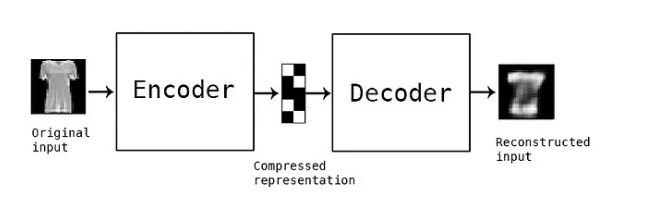
\includegraphics[width=1\textwidth]{figs/ejem_encoder_decoder.png}
  \captionof{figure}{Red feed forward}
  \label{fig-autoencoder}
\end{Figura}

Entrenaremos el autoencoder base con los siguientes hiperparámetros:
\begin{itemize}
  \item [-] $n = 64$.
  \item [-] $lr = 0.001$.
  \item [-] $p = 0.2$ (probabilidad de dropout).
  \item [-] $epochs = 15$.
  \item [-] $batch\_size = 100$.
  \item [-] $loss = MSELoss$.
  \item [-] $optimizer = Adam$.
\end{itemize}

La arquitectura del encoder es la siguiente:
\begin{itemize}
  \item Una capa convolucional 2D compuesta por:
  \begin{itemize}
    \item [-] un capa $Conv2d$ de entrada de dimensiones $(1, 28, 28)$ y de 
    salida $(16, 26, 26)$.
    \item [-] una capa de activación $ReLU$.
    \item [-] una capa $Dropout$.
    \item [-] una capa $MaxPool2d$, la cual mapea dimensiones $(16, 26, 26)$ a
    $(16, 13, 13)$.
  \end{itemize}
  \item Otra capa convolucional 2D compuesta por:
  \begin{itemize}
    \item [-] un capa $Conv2d$ de entrada de dimensiones $(16, 13, 13)$ y de 
    salida $(32, 11, 11)$
    \item [-] una capa de activación $ReLU$.
    \item [-] una capa $Dropout$.
    \item [-] una capa $MaxPool2d$, la cual mapea dimensiones $(32, 11, 11)$ a
    $(32, 5, 5)$.
  \end{itemize}
  \item Una capa lineal compuesta por:
  \begin{itemize}
    \item [-] una capa $Flatten$ que mapea dimensiones $(32, 5, 5)$ a $(800)$.
    \item [-] una capa $Linear$ de entrada $(800)$ y salida $n$.
    \item [-] una capa de activación $ReLU$.
    \item [-] una capa $Dropout$.
  \end{itemize}
\end{itemize}

El decoder con las siguientes capas:
\begin{itemize}
  \item Una capa lineal compuesta por:
  \begin{itemize}
    \item [-] una capa $Linear$ de entrada $n$ y salida $(800)$.
    \item [-] una capa de activación $ReLU$.
    \item [-] una capa $Dropout$.
    \item [-] una capa $Unflatten$ que mapea dimensiones $(800)$ a $(32, 5, 5)$.
  \end{itemize}
  \item Una capa convolucional 2D compuesta por:
  \begin{itemize}
    \item [-] un capa $ConvTranspose2d$ que mapea dimensiones $(32, 5, 5)$ a
    $(16, 13, 13)$.
    \item [-] una capa de activación $ReLU$.
    \item [-] una capa $Dropout$.
  \end{itemize}
  \item Otra capa convolucional 2D compuesta por:
  \begin{itemize}
    \item [-] un capa $ConvTranspose2d$ que mapea dimensione $(16, 13, 13)$ a
    $(1, 28, 28)$.
    \item [-] una capa de activación $Sigmoid$.
    \item [-] una capa $Dropout$.
  \end{itemize}
\end{itemize}

Luego variaremos los hiperparámetros de la red para ver como afecta su 
desempeño. Primero cambiaremos el optimizador por SGD, luego la probabilidad 
de dropout a $0.5$ y $0.1$. Siempre manteniendo el resto de los hiperparámetros
constantes para poder comparar los resultados.

\section{Clasificador Convolucional}
Una vez entrenado el autoencoder, procederemos a reutilizar el encoder para
entrenar un clasificador convolucional. La idea es que el encoder ya tiene
una buena representación de las imágenes, por lo que no es necesario volver a
entrenarlo.

El clasificador tendrá la siguiente arquitectura:
\begin{itemize}
  \item Una capa lineal compuesta por:
  \begin{itemize}
    \item [-] una capa $Linear$ de entrada $n$ y salida $10$.
    \item [-] una capa de activación $ReLU$.
    \item [-] una capa $Dropout$.
  \end{itemize}
\end{itemize}

Lo entrenaremos usando como base el modelo original y posteriormente solo 
reentrenaremos los parámetros de la capa clasificadora dejando los parámetros
de la capa codificadora tal como vienen entrenados del autoencoder convolucional.

\section{Resultados}
\subsection{Modelo sin entrenar}

En la figura \ref{fig-model-sin_entrenar} se muestra la imagen a predecir y las
imagenes reconstruidas por el modelo sin entrenar. Se puede observar que el
modelo no es capaz de reconstruir la imagen original.

\begin{Figura}
  \centering
  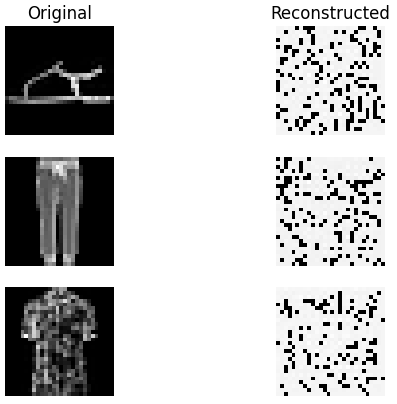
\includegraphics[width=0.5\textwidth]{figs/modelo_sin_entrenar.png}
  \captionof{figure}{Imagenea a predir vs imagenes reconstruidas por el modelo 
  sin entrenar}
  \label{fig-model-sin-entrenar}
\end{Figura}

\subsection{Modelo base entrenado}

Los resultados obtenidos para el modelo base entrenado se presentan en la figura
\ref{fig-modelb-entrenado-perdida}. Se ve que las curvas muestran una 
disminución en la función de pérdida a medida que avanzan las épocas, lo cual 
indica que le modelo mejora su capacidad de ajuste a los datos. Que las curvas 
sean casi identicas sugiere que no hay overfitting.
\begin{Figura}
  \centering
  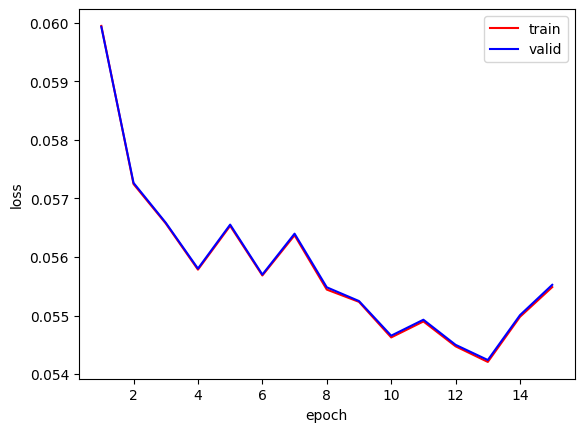
\includegraphics[width=0.60\textwidth]{figs/modelo_original.png}
  \captionof{figure}{Función de pérdida del modelo base entrenado}
  \label{fig-modelb-entrenado-perdida}
\end{Figura}

También se muestra en la figura \ref{fig-modelb-entrenado-img} la imagen a
predecir y las imagenes reconstruidas por el modelo base entrenado. Se puede
observar que el modelo es capaz de reconstruir la imagen original con un error
de reconstrucción menor.
\begin{Figura}
  \centering
  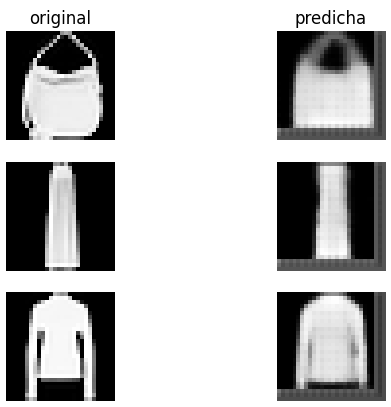
\includegraphics[width=0.5\textwidth]{figs/test_modelo_original.png}
  \captionof{figure}{Imagenea a predir vs imagenes reconstruidas por el modelo
  base entrenado}
  \label{fig-modelb-entrenado-img}
\end{Figura}

\subsection{Modelo con optimizador SGD}

Los resultados obtenidos para el modelo con optimizador SGD se presentan en la
figura \ref{fig-model-sgd} Se ve que las curvas muestran una gran disminución 
al inicio (epocas 0-10), con una posterior estabilización y un ligero aumento 
hacia el final despues de la epoca 20. Esto podria ser un signo de sobre ajuste,
donde el modelo comienza a ajustarse demaciado a los datos y pierde su capacidad
de generalización.

\begin{Figura}
  \centering
  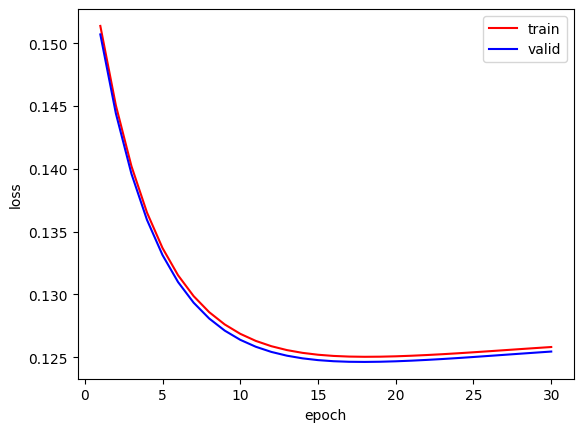
\includegraphics[width=0.60\textwidth]{figs/modelo_con_sdg.png}
  \captionof{figure}{Función de pérdida del modelo con optimizador SGD}
  \label{fig-model-sgd}
\end{Figura}

En el caso de la imagen a predecir y las imagenes reconstruidas por el modelo
con optimizador SGD se muestra en la figura \ref{fig-model-sgdb}. Se puede
observar que el modelo no es capaz de reconstruir la imagen original.

\begin{Figura}
  \centering
  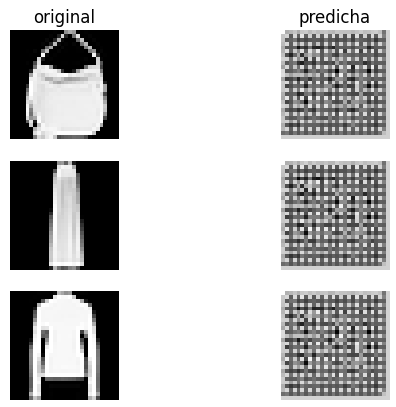
\includegraphics[width=0.5\textwidth]{figs/test_modelo_sdg.png}
  \captionof{figure}{Imagenea a predir vs imagenes reconstruidas por el modelo SDG}
  \label{fig-model-sgdb}
\end{Figura}

\subsection{Modelo con probabilidad de dropout 0.5, optimizador Adam}

En la figura \ref{fig-model-dropout05} se muestra la función de pérdida del
modelo con probabilidad de dropout 0.5. Se ve que las curvas muestran una 
oscilación en la función de pérdida a medida que avanzan las épocas, lo cual
indica que le modelo no mejora su capacidad de ajuste a los datos ya que la 
tasa de aprendizaje es muy alta produciendo ruido en el ajuste.

\begin{Figura}
  \centering
  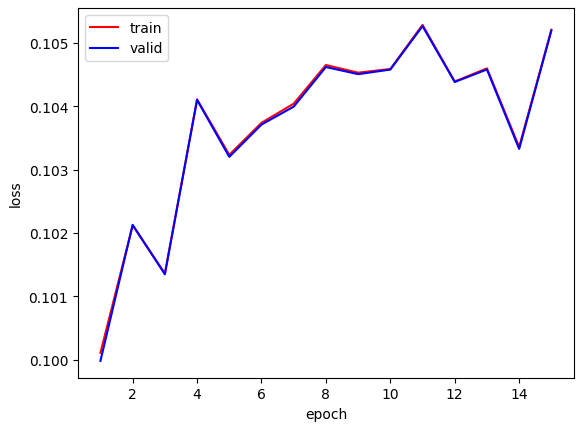
\includegraphics[width=0.60\textwidth]{figs/modelo_dropout05.png}
  \captionof{figure}{Función de pérdida del modelo con probabilidad de dropout 0.5}
  \label{fig-model-dropout05}
\end{Figura}

En la figura \ref{fig-model-dropout05b} las imágenes en la columna "predicha" 
parecen tener menos detalles en comparación con las originales, indicando que 
el modelo tiene dificultades para capturar todas las características de las 
imágenes originales. Esto puede deberse a un modelo subentrenado, la 
regularización por dropout muy alta, o una capacidad limitada del modelo. 
El modelo es capaz de captar los patrones generales de las imágenes, 
pero pierde información de alto nivel, como los bordes o los detalles más finos.

\begin{Figura}
  \centering
  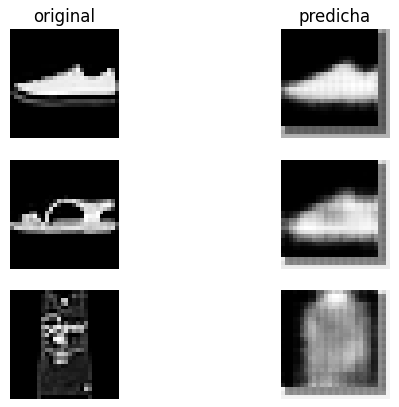
\includegraphics[width=0.5\textwidth]{figs/test_modelo_dropout05.png}
  \captionof{figure}{Imagenea a predir vs imagenes reconstruidas por el modelo
  con probabilidad de dropout 0.5}
  \label{fig-model-dropout05b}
\end{Figura}

\section{Clasificador Convolucional}

En esta sección se presentan los resultados obtenidos para el clasificador
convolucional que reutiliza el encoder del autoencoder previamente entrenado y 
en este caso se reentrenan todos los parámetros de la red por completo.

En la figura \ref{fig-clasificador-a} se muestra la función de pérdida del
modelo tomando como partida el modelo base, se observa que las curvas muestran
una disminución en la función de pérdida tanto en el conjunto de entrenamiento
como en el de validación a medida que avanzan las épocas, lo cual indica que le
modelo mejora su capacidad de ajuste a los datos, aun que hay fluctiaciones 
no se presentan signos de overfitting.

\begin{Figura}
  \centering
  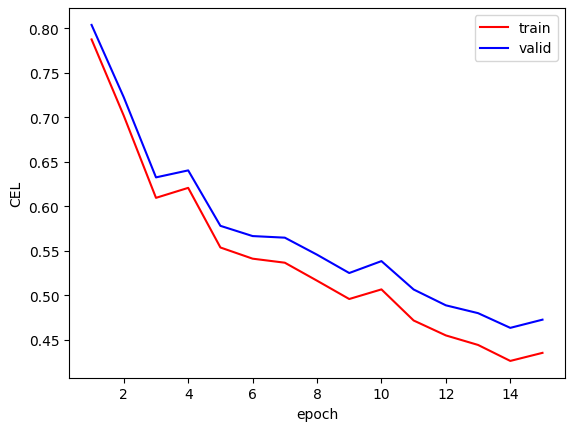
\includegraphics[width=0.60\textwidth]{figs/modelo_con_clasificador_a.png}
  \captionof{figure}{Función de pérdida del clasificador}
  \label{fig-clasificador-a}
\end{Figura}

La precisión aumenta en ambos conjuntos de datos segun se muestra en la figura
\ref{fig-clasificador-b}, lo cual indica que el modelo es capaz de generalizar
bien a partir de los datos de entrenamiento.

\begin{Figura}
  \centering
  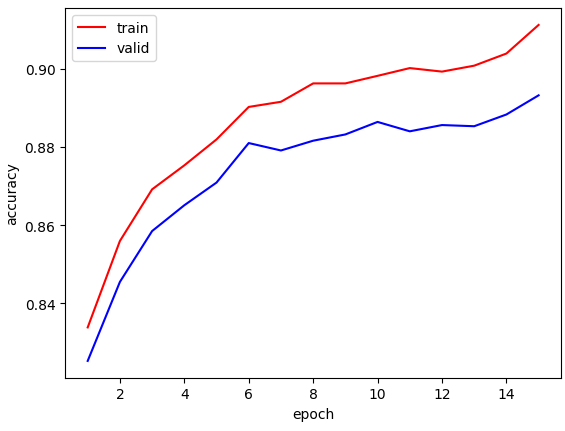
\includegraphics[width=0.60\textwidth]{figs/modelo_con_clasificador_b.png}
  \captionof{figure}{Presición del clasificador}
  \label{fig-clasificador-b}
\end{Figura}

Y la matriz de confución se muestra en la figura \ref{fig-matrix}, donde se 
puede observar un buen desempeño del clasificador. En la diagonal principal se
encuentran los valores más altos, lo cual indica que la mayoría de las
predicciones son correctas. Tiene un buen desempeño en clases como Sneaker, 
Bag, Trouser y Ankle Boot ya que sus valores de la diagonal principal esta 
en al valor mas alto de la escala cromatica. Pero tiene dificultades en 
distinguier entre las clases Shirt y Coat, ejemplo tomando la fila Shirt se ve 
que solo acierta 400 veces y 235 veces se equivoca prediciendo T-shirt y 245
como Pullover, algo similar ocurre con Coat, esto se debe a la similitud entre 
las categorías, ya que todas son prendas de vestir superiores.

\begin{Figura}
  \centering
  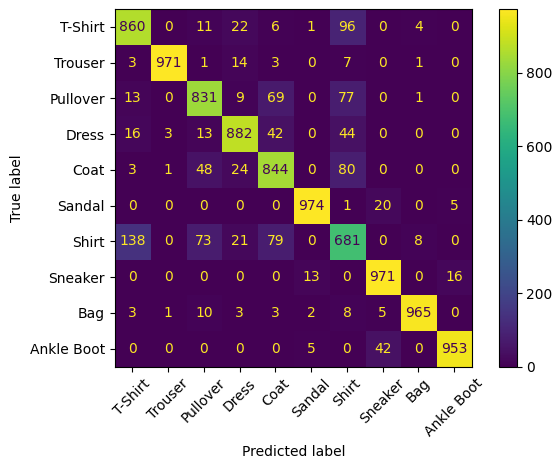
\includegraphics[width=0.75\textwidth]{figs/matrix_confuncion_modelo_con_clasificador.png}
  \captionof{figure}{Matriz de confución del clasificador}
  \label{fig-matrix}
\end{Figura}

\subsection{Clasificador solo entrenando la capa clasificadora}

Ahora analizamos los resultados obtenidos para el clasificador convolucional
reutilizando el encoder del autoencoder previamente entrenado y en este caso
solo reentrenando los parámetros de la capa clasificadora. Es decir, que 
tomando como punto de partida el modelo base, solo se reentrenan los parámetros
de la capa clasificadora.

En la figura \ref{fig-clasificador-a-a} se muestran las funciones de perdidas 
de ambos conjuntos de datos y se observa que las curvas muestran una disminución
bastante pronunciada en ambos casos. El comportamiento es similar al modelo
anterior.

\begin{Figura}
  \centering
  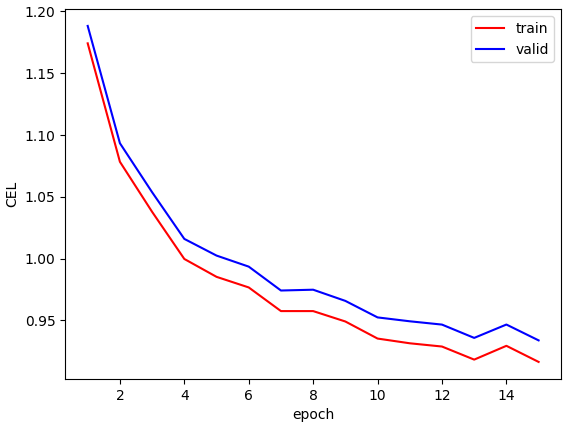
\includegraphics[width=0.60\textwidth]{figs/modelo_original_entrenando_solo_clasificadora_a.png}
  \captionof{figure}{Función de pérdida del clasificador - solo reentrenando la capa clasificadora}
  \label{fig-clasificador-a-a}
\end{Figura}

En la figura \ref{fig-clasificador-a-b} se muestra la precisión del modelo en
ambos conjuntos de datos. Se observa un comportamiento diferente al modelo 
anterior. Inicialmente ambas curvas aumentan, pero luego se estabilizan y 
comienzan a oscilar, esto puede ser un signo de sobre ajuste en el modelo.

\begin{Figura}
  \centering
  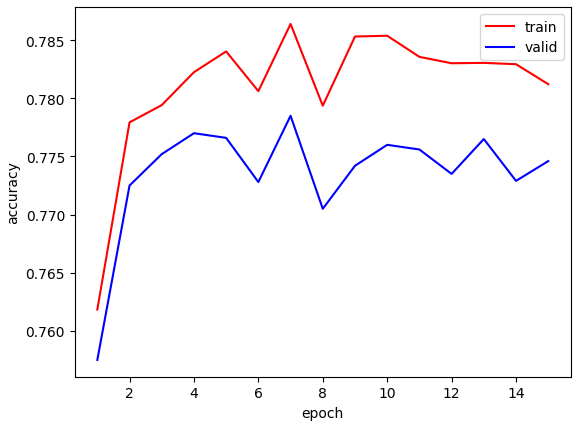
\includegraphics[width=0.60\textwidth]{figs/modelo_original_entrenando_solo_clasificadora_b.png}
  \captionof{figure}{Presición del clasificador - solo reentrenando la capa clasificadora}
  \label{fig-clasificador-a-b}
\end{Figura}

A fin de comparar el desempeño de ambos clasificadores, se muestra en la figura
\ref{fig-matrix-a} la matriz de confución donde efectivamente se comprueba que 
el desempeño del clasificador solo reentrenando la capa clasificadora es peor
que el modelo anterior. Ya que los valores de la diagonal principal son menores
en todos las categorias. Y además empeora mucho el desempeño en las categorias 
Coat y Shirt.

\begin{Figura}
  \centering
  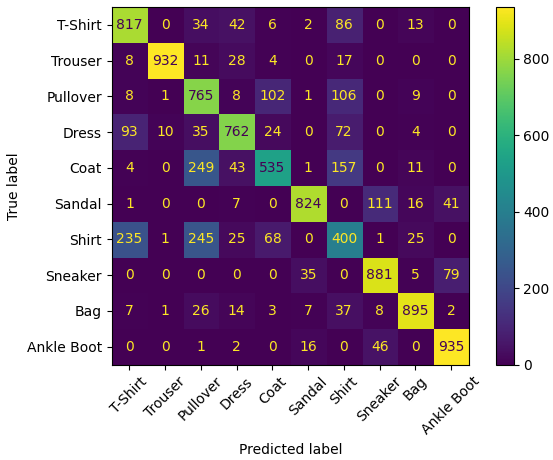
\includegraphics[width=0.75\textwidth]{figs/matrix_confucion_modelo_original_entrenando_solo_clasificadora.png}
  \captionof{figure}{matrix de confución - solo reentrenando la capa clasificadora}
  \label{fig-matrix-a}
\end{Figura}

Entonces podemos concluir que el modelo base donde se reentrenan todos los
parámetros de la red tiene un mejor desempeño que el modelo donde solo se
reentrenan los parámetros de la capa clasificadora.

\section{Conclusiones}

A lo largo de este trabajo se fueron entrenando diferentes modelos de redes
neuronales convolucionales. Se comenzó con un autoencoder convolucional,
luego se reutilizó el encoder para entrenar un clasificador convolucional y
finalmente se reentrenó solo la capa clasificadora.

A medida que se fue aumentado la complejidad de los modelos los resultados
fueron mejorando, sin embargo se observó que las distancias entre las curvas
de entrenamiento y validación se fueron agrandando, lo cual indica que los
modelos estaban sobreajustando los datos.

El modelos bases generaron buenos resultados tanto en el caso del autoencoder 
como en el clasificador. Y se pudo notar que al variar hiperparametros como el
optimizador, dropout hay que ser bastante cuidadoso ya que los resultados 
pueden variar mucho y no siempre para mejor. Asi como también en el caso 
de reentrenar solo la capa clasificadora, se observó que el modelo no
mejoró su desempeño sino que empeoró.

Algo muy importante a resaltar es que no es necesario entrenar los modelos 
durante muchas épocas, ya que con 15 épocas se obtuvieron resultados 
satisfactorios.

\bibliography{ref}

% Specify following sections are appendices. Use \appendix* if there
% only one appendix.

%\onecolumngrid


\end{document}
%
% ****** End of file apstemplate.tex ******